\documentclass[twoside]{book}

% Packages required by doxygen
\usepackage{fixltx2e}
\usepackage{calc}
\usepackage{doxygen}
\usepackage{graphicx}
\usepackage[utf8]{inputenc}
\usepackage{makeidx}
\usepackage{multicol}
\usepackage{multirow}
\PassOptionsToPackage{warn}{textcomp}
\usepackage{textcomp}
\usepackage[nointegrals]{wasysym}
\usepackage[table]{xcolor}

% Font selection
\usepackage[T1]{fontenc}
\usepackage{mathptmx}
\usepackage[scaled=.90]{helvet}
\usepackage{courier}
\usepackage{amssymb}
\usepackage{sectsty}
\renewcommand{\familydefault}{\sfdefault}
\allsectionsfont{%
  \fontseries{bc}\selectfont%
  \color{darkgray}%
}
\renewcommand{\DoxyLabelFont}{%
  \fontseries{bc}\selectfont%
  \color{darkgray}%
}
\newcommand{\+}{\discretionary{\mbox{\scriptsize$\hookleftarrow$}}{}{}}

% Page & text layout
\usepackage{geometry}
\geometry{%
  a4paper,%
  top=2.5cm,%
  bottom=2.5cm,%
  left=2.5cm,%
  right=2.5cm%
}
\tolerance=750
\hfuzz=15pt
\hbadness=750
\setlength{\emergencystretch}{15pt}
\setlength{\parindent}{0cm}
\setlength{\parskip}{0.2cm}
\makeatletter
\renewcommand{\paragraph}{%
  \@startsection{paragraph}{4}{0ex}{-1.0ex}{1.0ex}{%
    \normalfont\normalsize\bfseries\SS@parafont%
  }%
}
\renewcommand{\subparagraph}{%
  \@startsection{subparagraph}{5}{0ex}{-1.0ex}{1.0ex}{%
    \normalfont\normalsize\bfseries\SS@subparafont%
  }%
}
\makeatother

% Headers & footers
\usepackage{fancyhdr}
\pagestyle{fancyplain}
\fancyhead[LE]{\fancyplain{}{\bfseries\thepage}}
\fancyhead[CE]{\fancyplain{}{}}
\fancyhead[RE]{\fancyplain{}{\bfseries\leftmark}}
\fancyhead[LO]{\fancyplain{}{\bfseries\rightmark}}
\fancyhead[CO]{\fancyplain{}{}}
\fancyhead[RO]{\fancyplain{}{\bfseries\thepage}}
\fancyfoot[LE]{\fancyplain{}{}}
\fancyfoot[CE]{\fancyplain{}{}}
\fancyfoot[RE]{\fancyplain{}{\bfseries\scriptsize Generated on Sun Nov 13 2016 23\+:13\+:57 for My Project by Doxygen }}
\fancyfoot[LO]{\fancyplain{}{\bfseries\scriptsize Generated on Sun Nov 13 2016 23\+:13\+:57 for My Project by Doxygen }}
\fancyfoot[CO]{\fancyplain{}{}}
\fancyfoot[RO]{\fancyplain{}{}}
\renewcommand{\footrulewidth}{0.4pt}
\renewcommand{\chaptermark}[1]{%
  \markboth{#1}{}%
}
\renewcommand{\sectionmark}[1]{%
  \markright{\thesection\ #1}%
}

% Indices & bibliography
\usepackage{natbib}
\usepackage[titles]{tocloft}
\setcounter{tocdepth}{3}
\setcounter{secnumdepth}{5}
\makeindex

% Hyperlinks (required, but should be loaded last)
\usepackage{ifpdf}
\ifpdf
  \usepackage[pdftex,pagebackref=true]{hyperref}
\else
  \usepackage[ps2pdf,pagebackref=true]{hyperref}
\fi
\hypersetup{%
  colorlinks=true,%
  linkcolor=blue,%
  citecolor=blue,%
  unicode%
}

% Custom commands
\newcommand{\clearemptydoublepage}{%
  \newpage{\pagestyle{empty}\cleardoublepage}%
}


%===== C O N T E N T S =====

\begin{document}

% Titlepage & ToC
\hypersetup{pageanchor=false,
             bookmarks=true,
             bookmarksnumbered=true,
             pdfencoding=unicode
            }
\pagenumbering{roman}
\begin{titlepage}
\vspace*{7cm}
\begin{center}%
{\Large My Project }\\
\vspace*{1cm}
{\large Generated by Doxygen 1.8.8}\\
\vspace*{0.5cm}
{\small Sun Nov 13 2016 23:13:57}\\
\end{center}
\end{titlepage}
\clearemptydoublepage
\tableofcontents
\clearemptydoublepage
\pagenumbering{arabic}
\hypersetup{pageanchor=true}

%--- Begin generated contents ---
\chapter{Class Index}
\section{Class List}
Here are the classes, structs, unions and interfaces with brief descriptions\+:\begin{DoxyCompactList}
\item\contentsline{section}{\hyperlink{class_juego_de_la_vida}{Juego\+De\+La\+Vida} }{\pageref{class_juego_de_la_vida}}{}
\end{DoxyCompactList}

\chapter{Class Documentation}
\hypertarget{class_edge}{\section{Edge$<$ type $>$ Class Template Reference}
\label{class_edge}\index{Edge$<$ type $>$@{Edge$<$ type $>$}}
}


Collaboration diagram for Edge$<$ type $>$\+:
\nopagebreak
\begin{figure}[H]
\begin{center}
\leavevmode
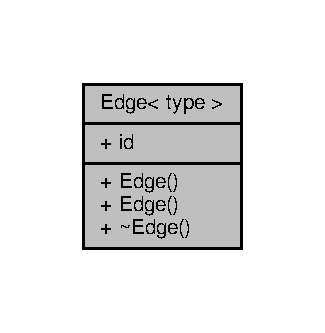
\includegraphics[width=156pt]{class_edge__coll__graph}
\end{center}
\end{figure}
\subsection*{Public Member Functions}
\begin{DoxyCompactItemize}
\item 
\hypertarget{class_edge_ab43f91be57927f083a0667624f8ce10e}{{\bfseries Edge} (type $\ast$name)}\label{class_edge_ab43f91be57927f083a0667624f8ce10e}

\end{DoxyCompactItemize}
\subsection*{Public Attributes}
\begin{DoxyCompactItemize}
\item 
\hypertarget{class_edge_acc1a8bc0a7119feb91e359fb15fc4a75}{type $\ast$ {\bfseries id}}\label{class_edge_acc1a8bc0a7119feb91e359fb15fc4a75}

\end{DoxyCompactItemize}


The documentation for this class was generated from the following file\+:\begin{DoxyCompactItemize}
\item 
Edge.\+h\end{DoxyCompactItemize}

\hypertarget{class_grafo}{\section{Grafo Class Reference}
\label{class_grafo}\index{Grafo@{Grafo}}
}


Collaboration diagram for Grafo\+:
\nopagebreak
\begin{figure}[H]
\begin{center}
\leavevmode
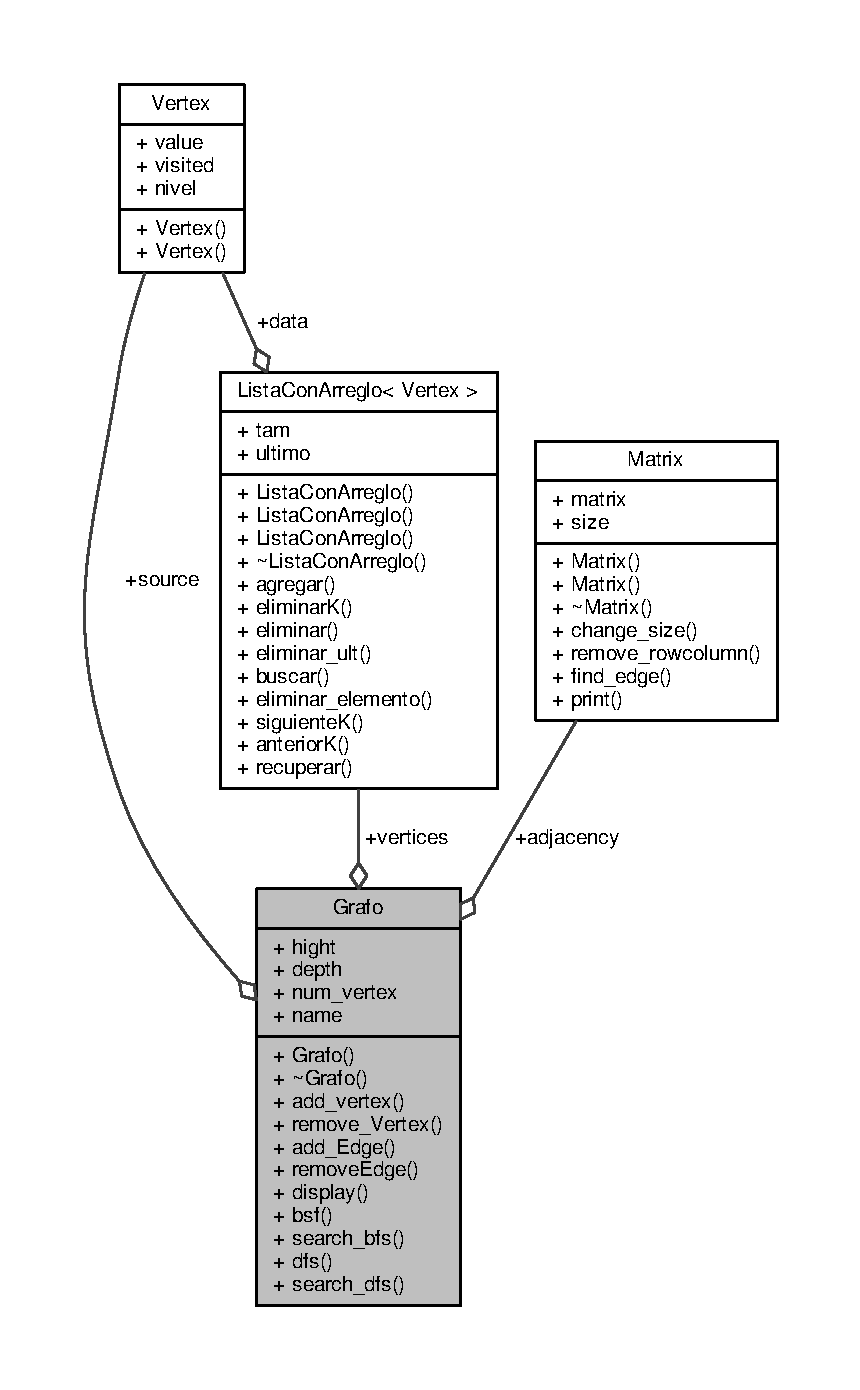
\includegraphics[height=550pt]{class_grafo__coll__graph}
\end{center}
\end{figure}
\subsection*{Public Member Functions}
\begin{DoxyCompactItemize}
\item 
\hypertarget{class_grafo_a3972f2c3bba286846dc48a63e49c638f}{void {\bfseries add\+\_\+vertex} (char $\ast$v)}\label{class_grafo_a3972f2c3bba286846dc48a63e49c638f}

\item 
\hypertarget{class_grafo_af798c61940a5fa26f160527c6f1ce800}{void {\bfseries remove\+\_\+\+Vertex} (\hyperlink{class_vertex}{Vertex} v)}\label{class_grafo_af798c61940a5fa26f160527c6f1ce800}

\item 
\hypertarget{class_grafo_ae1e62139433ab16cab3373e081e5f550}{void {\bfseries add\+\_\+\+Edge} (\hyperlink{class_vertex}{Vertex} v1, \hyperlink{class_vertex}{Vertex} v2)}\label{class_grafo_ae1e62139433ab16cab3373e081e5f550}

\item 
\hypertarget{class_grafo_ab9e96aabff359c0fec42179fe9a7d399}{void {\bfseries remove\+Edge} (int e)}\label{class_grafo_ab9e96aabff359c0fec42179fe9a7d399}

\item 
\hypertarget{class_grafo_a7fe03adf9aa8c7a316c23d29a49a9656}{void {\bfseries display} ()}\label{class_grafo_a7fe03adf9aa8c7a316c23d29a49a9656}

\item 
\hypertarget{class_grafo_af2826ab22e0e0fd540e1e846fdb2f7b9}{void {\bfseries bsf} ()}\label{class_grafo_af2826ab22e0e0fd540e1e846fdb2f7b9}

\item 
\hypertarget{class_grafo_a5c8a97350ac29ca22fca595e6b7e0d8f}{void {\bfseries search\+\_\+bfs} (int row, int column)}\label{class_grafo_a5c8a97350ac29ca22fca595e6b7e0d8f}

\item 
\hypertarget{class_grafo_a05a8f2152dd30308ca6ae5ec1227b5c3}{void {\bfseries dfs} ()}\label{class_grafo_a05a8f2152dd30308ca6ae5ec1227b5c3}

\item 
\hypertarget{class_grafo_aa75699ac87ede7cc285f4ce926e3d2df}{void {\bfseries search\+\_\+dfs} (int row, int column)}\label{class_grafo_aa75699ac87ede7cc285f4ce926e3d2df}

\end{DoxyCompactItemize}
\subsection*{Public Attributes}
\begin{DoxyCompactItemize}
\item 
\hypertarget{class_grafo_a2243cfbcfea660a6687783a3c8753766}{int {\bfseries hight}}\label{class_grafo_a2243cfbcfea660a6687783a3c8753766}

\item 
\hypertarget{class_grafo_ab284ac0fb5c14d9674413fa0ef5beae9}{int {\bfseries depth}}\label{class_grafo_ab284ac0fb5c14d9674413fa0ef5beae9}

\item 
\hypertarget{class_grafo_a27490ad976e4f9842df42be89647c5a3}{\hyperlink{class_vertex}{Vertex} $\ast$ {\bfseries source}}\label{class_grafo_a27490ad976e4f9842df42be89647c5a3}

\item 
\hypertarget{class_grafo_a2d8334d243cc65e35b37549b8e4f1244}{int {\bfseries num\+\_\+vertex}}\label{class_grafo_a2d8334d243cc65e35b37549b8e4f1244}

\item 
\hypertarget{class_grafo_a0f3fd7c3cd439278b331d799edaa5295}{\hyperlink{class_lista_con_arreglo}{Lista\+Con\+Arreglo}$<$ \hyperlink{class_vertex}{Vertex} $>$ $\ast$ {\bfseries vertices}}\label{class_grafo_a0f3fd7c3cd439278b331d799edaa5295}

\item 
\hypertarget{class_grafo_a83302ee3c077c1047fc48396e3d91f49}{\hyperlink{class_matrix}{Matrix} $\ast$ {\bfseries adjacency}}\label{class_grafo_a83302ee3c077c1047fc48396e3d91f49}

\item 
\hypertarget{class_grafo_a78acf4713466a323c53f6e549e8ec290}{int {\bfseries name}}\label{class_grafo_a78acf4713466a323c53f6e549e8ec290}

\end{DoxyCompactItemize}


The documentation for this class was generated from the following files\+:\begin{DoxyCompactItemize}
\item 
Grafo.\+h\item 
Grafo.\+cpp\end{DoxyCompactItemize}

\hypertarget{class_lista}{\section{Lista$<$ T $>$ Class Template Reference}
\label{class_lista}\index{Lista$<$ T $>$@{Lista$<$ T $>$}}
}


Inheritance diagram for Lista$<$ T $>$\+:
\nopagebreak
\begin{figure}[H]
\begin{center}
\leavevmode
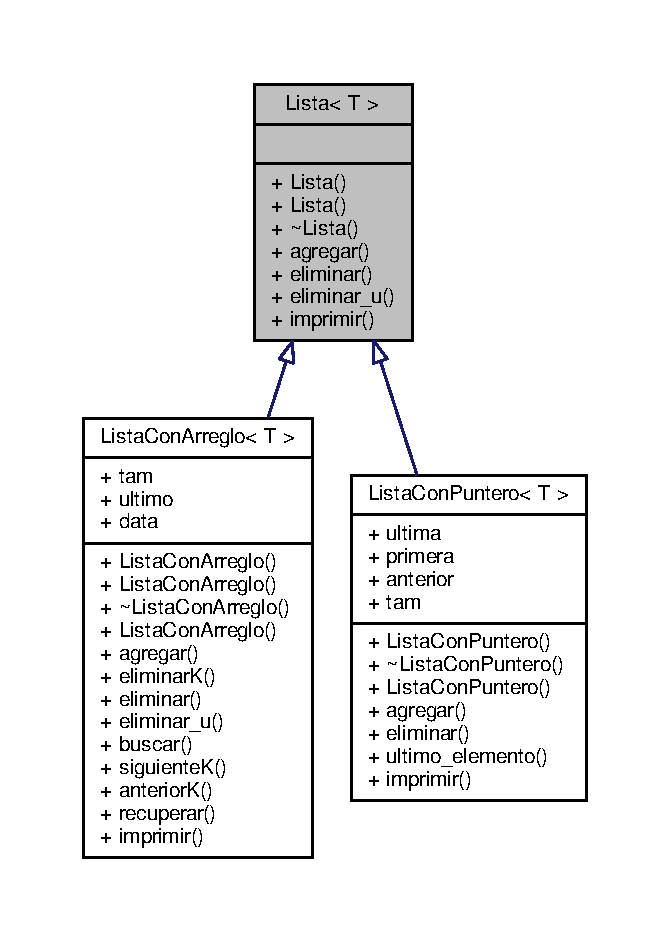
\includegraphics[width=322pt]{class_lista__inherit__graph}
\end{center}
\end{figure}


Collaboration diagram for Lista$<$ T $>$\+:
\nopagebreak
\begin{figure}[H]
\begin{center}
\leavevmode
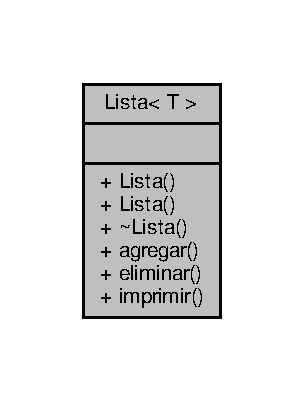
\includegraphics[width=156pt]{class_lista__coll__graph}
\end{center}
\end{figure}
\subsection*{Public Member Functions}
\begin{DoxyCompactItemize}
\item 
\hypertarget{class_lista_ad63a49df32595e2f321fffd7ffa1346a}{{\bfseries Lista} (const \hyperlink{class_lista}{Lista} \&orig)}\label{class_lista_ad63a49df32595e2f321fffd7ffa1346a}

\item 
\hypertarget{class_lista_aea57814c283f14cd0d31b8da37c622a9}{virtual void {\bfseries agregar} (T e)=0}\label{class_lista_aea57814c283f14cd0d31b8da37c622a9}

\item 
\hypertarget{class_lista_aabdd833f1bc38b8174838f92c5b438b3}{virtual void {\bfseries eliminar} ()=0}\label{class_lista_aabdd833f1bc38b8174838f92c5b438b3}

\item 
\hypertarget{class_lista_aa0da522793d55d38f5ba1faf4354b1df}{virtual void {\bfseries eliminar\+\_\+u} ()=0}\label{class_lista_aa0da522793d55d38f5ba1faf4354b1df}

\item 
\hypertarget{class_lista_af398229330911af031fc1d89a556a840}{virtual void {\bfseries imprimir} ()=0}\label{class_lista_af398229330911af031fc1d89a556a840}

\end{DoxyCompactItemize}


The documentation for this class was generated from the following file\+:\begin{DoxyCompactItemize}
\item 
Lista.\+h\end{DoxyCompactItemize}

\hypertarget{class_lista_con_arreglo}{\section{Lista\+Con\+Arreglo$<$ T $>$ Class Template Reference}
\label{class_lista_con_arreglo}\index{Lista\+Con\+Arreglo$<$ T $>$@{Lista\+Con\+Arreglo$<$ T $>$}}
}


Inheritance diagram for Lista\+Con\+Arreglo$<$ T $>$\+:
\nopagebreak
\begin{figure}[H]
\begin{center}
\leavevmode
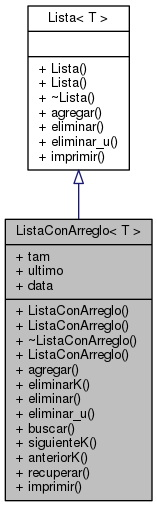
\includegraphics[width=190pt]{class_lista_con_arreglo__inherit__graph}
\end{center}
\end{figure}


Collaboration diagram for Lista\+Con\+Arreglo$<$ T $>$\+:
\nopagebreak
\begin{figure}[H]
\begin{center}
\leavevmode
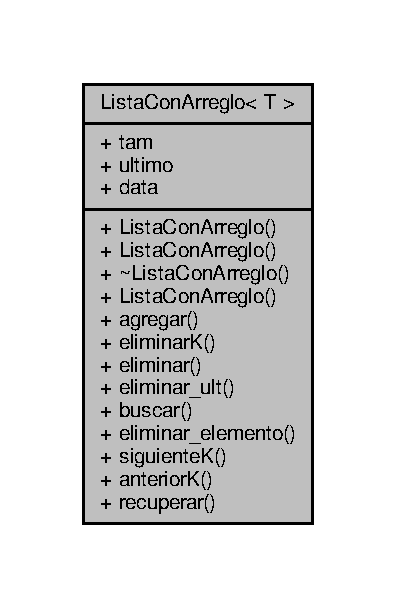
\includegraphics[width=190pt]{class_lista_con_arreglo__coll__graph}
\end{center}
\end{figure}
\subsection*{Public Member Functions}
\begin{DoxyCompactItemize}
\item 
\hypertarget{class_lista_con_arreglo_ab7a22a8f04de9403d32a7431d4dd9627}{{\bfseries Lista\+Con\+Arreglo} (const \hyperlink{class_lista_con_arreglo}{Lista\+Con\+Arreglo} \&orig)}\label{class_lista_con_arreglo_ab7a22a8f04de9403d32a7431d4dd9627}

\item 
\hypertarget{class_lista_con_arreglo_a9541812a0019b76c6529184356913a59}{{\bfseries Lista\+Con\+Arreglo} (int N)}\label{class_lista_con_arreglo_a9541812a0019b76c6529184356913a59}

\item 
\hypertarget{class_lista_con_arreglo_a5336f6ef59e2cfaa008c4ad8cbee9f25}{void {\bfseries agregar} (T e)}\label{class_lista_con_arreglo_a5336f6ef59e2cfaa008c4ad8cbee9f25}

\item 
\hypertarget{class_lista_con_arreglo_acd8b8f484dc440dc64dc58cad375e7e4}{void {\bfseries eliminar\+K} (int k)}\label{class_lista_con_arreglo_acd8b8f484dc440dc64dc58cad375e7e4}

\item 
\hypertarget{class_lista_con_arreglo_a1d4ea3c3bbefa8d2c12ea520e12f5f9c}{virtual void {\bfseries eliminar} ()}\label{class_lista_con_arreglo_a1d4ea3c3bbefa8d2c12ea520e12f5f9c}

\item 
\hypertarget{class_lista_con_arreglo_a9f0f4138dcf42e664213ffbcedce2056}{virtual void {\bfseries eliminar\+\_\+u} ()}\label{class_lista_con_arreglo_a9f0f4138dcf42e664213ffbcedce2056}

\item 
\hypertarget{class_lista_con_arreglo_af2fe968f5ec674cb9640e11a1bcaab99}{int {\bfseries buscar} (T e)}\label{class_lista_con_arreglo_af2fe968f5ec674cb9640e11a1bcaab99}

\item 
\hypertarget{class_lista_con_arreglo_a8a3d5d83291eeab7d9dbb2108a6942ea}{char {\bfseries siguiente\+K} (int k)}\label{class_lista_con_arreglo_a8a3d5d83291eeab7d9dbb2108a6942ea}

\item 
\hypertarget{class_lista_con_arreglo_a78e25313648f0d4f188f61f60d7ba4b6}{char {\bfseries anterior\+K} (int k)}\label{class_lista_con_arreglo_a78e25313648f0d4f188f61f60d7ba4b6}

\item 
\hypertarget{class_lista_con_arreglo_af880c9a6795cf9281f2a217d0a4b0c07}{T {\bfseries recuperar} (int k)}\label{class_lista_con_arreglo_af880c9a6795cf9281f2a217d0a4b0c07}

\item 
\hypertarget{class_lista_con_arreglo_aa8267cef7510ef79626a812b3c85505d}{void {\bfseries imprimir} ()}\label{class_lista_con_arreglo_aa8267cef7510ef79626a812b3c85505d}

\end{DoxyCompactItemize}
\subsection*{Public Attributes}
\begin{DoxyCompactItemize}
\item 
\hypertarget{class_lista_con_arreglo_a7b1a9c6334db75f4ffb023a95b01e3f4}{int {\bfseries tam}}\label{class_lista_con_arreglo_a7b1a9c6334db75f4ffb023a95b01e3f4}

\item 
\hypertarget{class_lista_con_arreglo_a41f052fbde3598cb6f7ec7d8412be8c3}{int {\bfseries ultimo}}\label{class_lista_con_arreglo_a41f052fbde3598cb6f7ec7d8412be8c3}

\item 
\hypertarget{class_lista_con_arreglo_af5771ddbfd5f2fbd5925cb5bae26908e}{T $\ast$ {\bfseries data}}\label{class_lista_con_arreglo_af5771ddbfd5f2fbd5925cb5bae26908e}

\end{DoxyCompactItemize}


The documentation for this class was generated from the following file\+:\begin{DoxyCompactItemize}
\item 
Lista\+Con\+Arreglo.\+h\end{DoxyCompactItemize}

\hypertarget{class_matrix}{\section{Matrix Class Reference}
\label{class_matrix}\index{Matrix@{Matrix}}
}


Collaboration diagram for Matrix\+:
\nopagebreak
\begin{figure}[H]
\begin{center}
\leavevmode
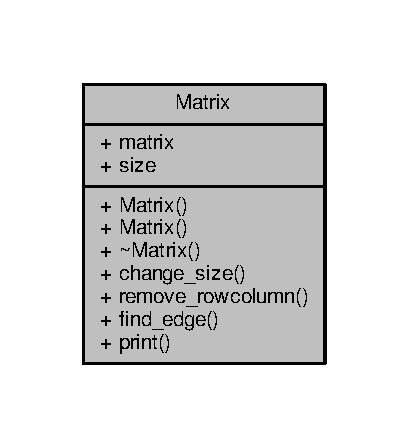
\includegraphics[width=196pt]{class_matrix__coll__graph}
\end{center}
\end{figure}
\subsection*{Public Member Functions}
\begin{DoxyCompactItemize}
\item 
\hypertarget{class_matrix_ae763d5a5d65e3c0f185bebd7766124ba}{{\bfseries Matrix} (int tam)}\label{class_matrix_ae763d5a5d65e3c0f185bebd7766124ba}

\item 
\hypertarget{class_matrix_ae1235f5c15ae98654e92ea2661ca60ea}{{\bfseries Matrix} (int $\ast$$\ast$values, int tam)}\label{class_matrix_ae1235f5c15ae98654e92ea2661ca60ea}

\item 
\hypertarget{class_matrix_a1e9a500f0ca4e681153fee9b2727b836}{void {\bfseries change\+\_\+size} (int new\+\_\+size)}\label{class_matrix_a1e9a500f0ca4e681153fee9b2727b836}

\item 
\hypertarget{class_matrix_a8360b94a374a116db0cc9163467ac4d7}{void {\bfseries remove\+\_\+rowcolumn} (int row)}\label{class_matrix_a8360b94a374a116db0cc9163467ac4d7}

\item 
\hypertarget{class_matrix_a63682775de6a8d35bc89cabbc35e2d61}{int $\ast$ {\bfseries find\+\_\+edge} (int e)}\label{class_matrix_a63682775de6a8d35bc89cabbc35e2d61}

\item 
\hypertarget{class_matrix_a99ba97122b8fdd54e95290caf80fc8e2}{void {\bfseries print} ()}\label{class_matrix_a99ba97122b8fdd54e95290caf80fc8e2}

\end{DoxyCompactItemize}
\subsection*{Public Attributes}
\begin{DoxyCompactItemize}
\item 
\hypertarget{class_matrix_a0df8ee2a361c4d678fcde2fcf3a8e4f9}{int $\ast$$\ast$ {\bfseries matrix}}\label{class_matrix_a0df8ee2a361c4d678fcde2fcf3a8e4f9}

\item 
\hypertarget{class_matrix_acd4947d87d17f777df33e32cef2e873c}{int {\bfseries size}}\label{class_matrix_acd4947d87d17f777df33e32cef2e873c}

\end{DoxyCompactItemize}


The documentation for this class was generated from the following files\+:\begin{DoxyCompactItemize}
\item 
Matrix.\+h\item 
Matrix.\+cpp\end{DoxyCompactItemize}

\hypertarget{class_vertex}{\section{Vertex Class Reference}
\label{class_vertex}\index{Vertex@{Vertex}}
}


Collaboration diagram for Vertex\+:
\nopagebreak
\begin{figure}[H]
\begin{center}
\leavevmode
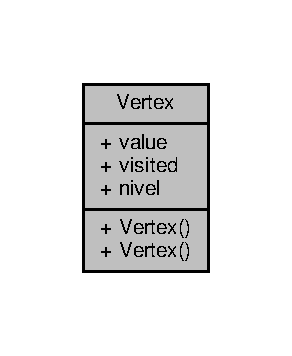
\includegraphics[width=140pt]{class_vertex__coll__graph}
\end{center}
\end{figure}
\subsection*{Public Member Functions}
\begin{DoxyCompactItemize}
\item 
\hypertarget{class_vertex_a30feb00a36bf5da73c84056a0aa1c7eb}{{\bfseries Vertex} (bool visit, char $\ast$val)}\label{class_vertex_a30feb00a36bf5da73c84056a0aa1c7eb}

\end{DoxyCompactItemize}
\subsection*{Public Attributes}
\begin{DoxyCompactItemize}
\item 
\hypertarget{class_vertex_a05c7844feef250d9a319ac49d1dbdfa4}{char $\ast$ {\bfseries value}}\label{class_vertex_a05c7844feef250d9a319ac49d1dbdfa4}

\item 
\hypertarget{class_vertex_aaef9f7de91b4b8f1752d391a1aae9c2e}{bool {\bfseries visited}}\label{class_vertex_aaef9f7de91b4b8f1752d391a1aae9c2e}

\item 
\hypertarget{class_vertex_a7fc49a2ab06e5d4cad86278c65303fc2}{int {\bfseries nivel}}\label{class_vertex_a7fc49a2ab06e5d4cad86278c65303fc2}

\end{DoxyCompactItemize}


The documentation for this class was generated from the following files\+:\begin{DoxyCompactItemize}
\item 
Vertex.\+h\item 
Vertex.\+cpp\end{DoxyCompactItemize}

%--- End generated contents ---

% Index
\newpage
\phantomsection
\addcontentsline{toc}{chapter}{Index}
\printindex

\end{document}
